\chapter{Imaging systems}
\label{app:ImagingSystems}


\section{Geometric optics of imaging systems}
Let the optical axis of an arbitrary optical system lie along the $z$-axis,
and let all optical rays lie in a plane with the optical axis.
At a given position $z_j$, an optical ray is fully described by
its transverse distance $\rho$ to the optical axis and
its slope $d\rho / dz$.
In the paraxial limit $d\rho / dz \approx \theta$,
where $\theta$ is the angle between the ray and the optical axis.
Ray propagation through homogeneous media and refractive interfaces
is well-governed by the so-called $ABCD$ ray-matrix formalism
\cite[Ch.~15]{siegman_lasers};
that is, a ray propagating from point $j$ to point $j + 1$ evolves as
\begin{equation}
  \begin{pmatrix}
    \rho_{j + 1}
    \\
    \theta_{j + 1}
  \end{pmatrix}
  =
  \begin{pmatrix}
    A & B
    \\
    C & D
  \end{pmatrix}
  \begin{pmatrix}
    \rho_j
    \\
    \theta_j
  \end{pmatrix},
  \label{eq:ImagingSystems:ABCD_ray_tracing_general}
\end{equation}
where the $ABCD$ matrix elements are determined
by the optical properties of the media between points $j$ and $j + 1$.
Some rudimentary $ABCD$ matrices are given in
Table~\ref{table:ImagingSystems:ABCD_matrices}, while
more exhaustive lists can be readily found elsewhere
\cite[Ch.~15]{siegman_lasers}~\cite{tovar_generalized_beam_matrices_IV}.

\begin{table}
  \centering
  \renewcommand{\arraystretch}{1.5}% Spread rows out...
  \begin{tabular}{%
    >{\centering}m{6cm} >{\centering}m{4.5cm}
  }
    \toprule%
    \textbf{optical element} & $\mathbf{ABCD}$~\textbf{matrix}
    \tabularnewline%
    \midrule
    \textbf{propagation} by distance $d$ \\
    through medium of constant \\
    index of refraction, $N$
    &
    $\begin{pmatrix}
      1 & d
      \\
      \phantom{-} 0 \phantom{f} & 1  % phantoms to match thin lens format
    \end{pmatrix}$
    \tabularnewline%
    \textbf{thin lens} with \\
    focal length $f$
    &
    $\begin{pmatrix}
      1 & 0
      \\
      -1/f & 1
    \end{pmatrix}$
    \tabularnewline%
    \toprule%
  \end{tabular}
  \caption[Some $ABCD$ ray matrices]{Some useful $ABCD$ ray matrices.}
\label{table:ImagingSystems:ABCD_matrices}
\end{table}

An imaging system $\image$, by definition,
redirects all rays emanating from transverse position $\rho_{\object}$
in the object plane $S_{\object}$
to intersect at transverse position
\begin{equation}
  \rho_{\image} = M \rho_{\object}
  \label{eq:ImagingSystems:image_plane_transverse_coordinates}
\end{equation}
in the image plane $S_{\image}$.
Here, $M$ is the \emph{magnification} of the imaging system, and
$M < 0$ implies that the image is inverted relative to the object.
The imaging system's $A$, $B$, and $D$ matrix elements
are easily determined by inspection.
Recalling the ray-matrix definitions in
(\ref{eq:ImagingSystems:ABCD_ray_tracing_general}),
note that
$\rho_{\image} = M \rho_{\object} = A \rho_{\object} + B \theta_{\object}$
such that $A = M$ and $B = 0$.
Further, assuming the image plane and object plane refractive indices
are identical, as is often the case,
the determinant of the ray matrix is unity
(i.e.\ $AD - BC = 1$)~\cite{halbach_63}
such that $D = 1 / M$.
The final matrix element $C$ is determined by the particulars
of the imaging system;
for propagation through ``simple'' optical components,
such as lenses and homogeneous media, $C$ is constrained to be real.
Thus, an imaging system of magnification $M$ is characterized
by an $ABCD$ ray matrix of the form
\begin{equation}
  \mathcal{I}
  =
  \begin{pmatrix}
    M & 0
    \\
    C & 1 / M
  \end{pmatrix}.
  \label{eq:ImagingSystems:ABCD_imaging}
\end{equation}

The symmetry axis of a Gaussian beam
behaves as a ray in the geometric-optics sense
\cite{tovar_generalized_beam_matrices_IV}.
Application of the imaging $ABCD$ ray matrix
(\ref{eq:ImagingSystems:ABCD_imaging})
to a beam scattered by $\theta_m$ in the object plane
(i.e.\ see (\ref{eq:InterferometricMethods:scattered_beam_wavevector}))
indicates that this beam will be rotated by angle $\theta_m / M$
relative to the unscattered beam in the image plane,
as shown in Fig.~\ref{fig:ImagingSystems:imaging_geometry}.
Further, the imaging optics do \emph{not} alter
the magnitude of the beam's wavevector, i.e.\ $|\image(\vect{k}_m)| = k_0$
(this readily follows from the fact that the imaging optics
do not alter the energy of the beam's constituent photons).
Knowledge of the wavevector's image-plane magnitude and orientation
allows determination of the image-plane wavevector as
\begin{align}
  \image(\vect{k}_{0,m})
  =
  \vect{k}_{0,m,\image}
  =
  \left( m k_{\image} \right) \hat{\vect{x}}
  +
  k_0 \left[ 1 - \left(\frac{m k_{\image}}{k_0}\right)^2 \right]^{1/2}
  \hat{\vect{z}},
  \label{eq:ImagingSystems:scattered_beam_wavevector_image_plane}
\end{align}
where
\begin{equation}
  k_{\image} \equiv \frac{k}{M}
  \label{eq:ImagingSystems:image_plane_fluctuation_wavenumber}
\end{equation}
is the \emph{imaged} wavenumber
of the corresponding object-plane phase fluctuation
(\ref{eq:InterferometricMethods:cosine_phase_fluctuation}).

\begin{figure}
  \centering
  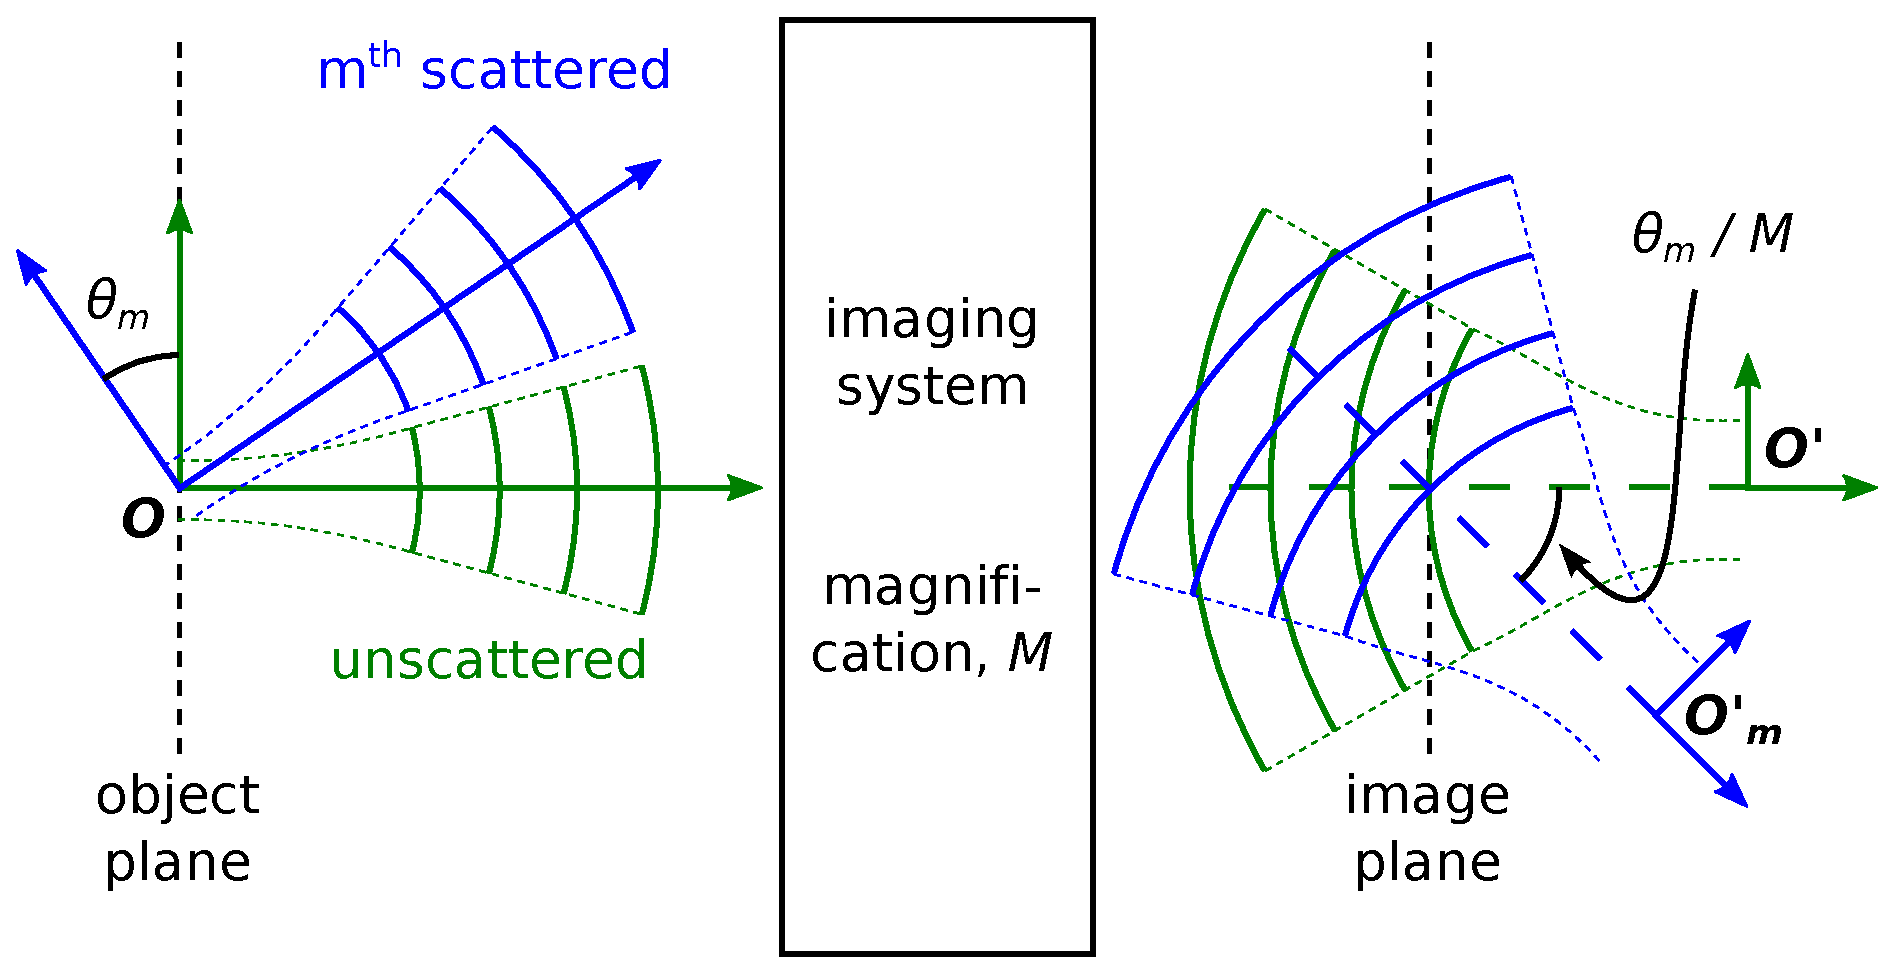
\includegraphics[width = \textwidth]{%
    Appendices/ImagingSystems/figs/imaging_geometry.eps}
  \caption[Imaging geometry]{%
    Beam geometries in an imaging system with magnification $M$.
    Beam scattering occurs in the object plane at the probe beam's waist.
    Thus, the $m$\ts{th} scattered beam
    shares the origin $\vect{O}_{\object}$ with the unscattered beam but
    is angularly separated by $\theta_m$.
    The imaging system redirects all beams emanating from $\vect{O}_{\object}$
    to intersect at angle $\theta_m / M$ in the image plane.
    In general, the image plane does \emph{not} sit at a beam waist
    such that the post-imaging-system beam waists
    of the scattered and unscattered beams do not coincide,
    i.e.\ $\vect{O}_{\image} \neq \vect{O}_{m,\image}$.}
\label{fig:ImagingSystems:imaging_geometry}
\end{figure}


\section{Gaussian-beam transformation in imaging systems}
\label{sec:ImagingSystems:imaging:Gaussian_beam_transformation}
In addition to manipulating the ray-like trajectory
of a Gaussian beam's symmetry axis,
an imaging system also alters
other important properties of an incident Gaussian beam.
A Gaussian beam is fully characterized by
its in-medium wavelength $\lambda_0 / N$,
its width $w(z_j)$, and
its radius of curvature $R(z_j)$
at a single location $z_j$.
These parameters can be conveniently combined
to define the so-called complex beam parameter $q$
\cite[Sec.~17.1]{siegman_lasers}
\begin{equation}
  \frac{1}{q}
  \equiv
  \frac{1}{R}
  -
  i \left( \frac{\lambda_0}{N \pi w^2} \right).
  \label{eq:ImagingSystems:complex_beam_parameter_inverse}
\end{equation}
Referencing the Gaussian-beam width
(\ref{eq:InterferometricMethods:Gaussian_beam_width}) and
the Gaussian-beam radius of curvature
(\ref{eq:InterferometricMethods:Gaussian_beam_radius_of_curvature}),
the complex beam parameter can be rewritten as
\begin{equation}
  q = z + i z_R,
  \label{eq:ImagingSystems:complex_beam_parameter}
\end{equation}
where $z$ is the axial distance from the beam waist and
$z_R$ is the Rayleigh range (\ref{eq:InterferometricMethods:Rayleigh_range}).
The Gaussian beam can then be propagated from point $j$ to point $j + 1$ via
\begin{equation}
  q_{j+1}
  =
  \frac{A q_j + B}{C q_j + D},
  \label{eq:ImagingSystems:complex_beam_parameter_propagation}
\end{equation}
where, amazingly, $A$, $B$, $C$, and $D$
are equal to the corresponding values
of the $ABCD$ ray matrix from geometric optics
\cite[Sec.~20.2]{siegman_lasers} \cite{tovar_generalized_beam_matrices_IV}.
The beam's transverse and angular displacements
relative to the lab-frame optical axis
are similarly governed by the so-called ``$S$-parameter transformation''
\cite{tovar_generalized_beam_matrices_IV}.
It is important to note that the complex beam parameter and its evolution
are \emph{independent} of the beam's transverse and angular displacements
from the lab-frame optical axis
(assuming such displacements do not violate the paraxial limit, of course);
that is, a scattered beam's width and radius of curvature
evolve identically to those of the unscattered beam.

The properties of the image-plane beams are easily determined.
Using the ray matrix of an imaging system from
(\ref{eq:ImagingSystems:ABCD_imaging}),
the image-plane complex beam parameter $q_{\image}$ is given as
\begin{equation}
  q_{\image}
  =
  \frac{M q_{\object}}{C q_{\object} + (1 / M)},
  \label{eq:ImagingSystems:complex_beam_parameter_image_plane}
\end{equation}
where $q_{\object}$ is the object-plane complex beam parameter,
and $M$ and $C$ are both real.
Note that the post-imaging-system beam waists
do \emph{not} necessarily sit at the image plane,
in which case the beams' native coordinate systems
are necessarily \emph{displaced} from each other
(i.e.\ $\vect{O}_{\image} \neq \vect{O}_{m,\image}$,
as indicated in Fig.~\ref{fig:ImagingSystems:imaging_geometry}).
Examining the image-plane complex beam parameter
(\ref{eq:ImagingSystems:complex_beam_parameter_image_plane})
it is easy to see that the beam waists will not sit at the image plane
when $|C q_{\object}| \gg 1 / M$ such that
$z_{\image} = \text{Re}(q_{\image}) \approx M / C \neq 0$.

As the native coordinate systems of
the unscattered beam and the $m$\ts{th} scattered beam
do not align in the image plane,
it will be convenient to determine the relevant coordinate transformation.
The transformation is derived for the most general case
in which the beam waists do not sit at the image plane
(i.e.\ $\vect{O}_{\image} \neq \vect{O}_{m,\image}$,
as indicated in Fig.~\ref{fig:ImagingSystems:imaging_geometry}).
The coordinate transformation is simply a series of translations and rotations
\begin{equation}
  \vect{r}_{m, \image}
  =
  \left[ \vect{R}(\theta_m / M) \right]
  \left[ \vect{r}_{\image} - z_{\image} \hat{\vect{z}} \right]
  +
  z_{\image} \hat{\vect{z}},
  \label{eq:ImagingSystems:coordinate_transformation_imaging_plane_compact}
\end{equation}
where
\begin{equation}
  \vect{R}(\theta)
  =
  \begin{pmatrix}
    \cos\theta & 0 & -\sin\theta
    \\
    0          & 1 & 0
    \\
    \sin\theta & 0 & \cos\theta
  \end{pmatrix}
  \label{eq:ImagingSystems:rotation_matrix}
\end{equation}
is the rotation matrix
that rotates the $(x, z)$-plane about the $y$-axis by angle $\theta$.
Explicitly, the image-plane coordinate transformation
(\ref{eq:ImagingSystems:coordinate_transformation_imaging_plane_compact}) is
\begin{equation}
  \begin{pmatrix}
    x_{m, \image}
    \\
    y_{m, \image}
    \\
    z_{m, \image}
  \end{pmatrix}
  =
  \begin{pmatrix}
    x_{\image} \cos\left( \frac{\theta_m}{M} \right)
    \\
    y_{\image}
    \\
    z_{\image} + x_{\image} \sin\left( \frac{\theta_m}{M} \right)
  \end{pmatrix}
  \approx
  \begin{pmatrix}
    x_{\image}
    \\
    y_{\image}
    \\
    z_{\image} + x_{\image} \left( \frac{\theta_m}{M} \right)
  \end{pmatrix},
  \label{eq:ImagingSystems:coordinate_transformation_imaging_plane}
\end{equation}
where the approximation is valid to first order in $\theta_m / M$.


\bibliographystyle{plainurl}
\bibliography{references}
